\documentclass[a4paper,]{article}
\usepackage{lmodern}
\usepackage{amssymb,amsmath}
\usepackage{ifxetex,ifluatex}
\usepackage{fixltx2e} % provides \textsubscript
\ifnum 0\ifxetex 1\fi\ifluatex 1\fi=0 % if pdftex
  \usepackage[T1]{fontenc}
  \usepackage[utf8]{inputenc}
\else % if luatex or xelatex
  \ifxetex
    \usepackage{mathspec}
  \else
    \usepackage{fontspec}
  \fi
  \defaultfontfeatures{Ligatures=TeX,Scale=MatchLowercase}
\fi
% use upquote if available, for straight quotes in verbatim environments
\IfFileExists{upquote.sty}{\usepackage{upquote}}{}
% use microtype if available
\IfFileExists{microtype.sty}{%
\usepackage{microtype}
\UseMicrotypeSet[protrusion]{basicmath} % disable protrusion for tt fonts
}{}
\usepackage[margin=1in]{geometry}
\usepackage{hyperref}
\hypersetup{unicode=true,
            pdftitle={Identifying key influences for planning acceptance of onshore wind turbines},
            pdfauthor={Michael Harper, Ben Anderson, Patrick James, AbuBakr Bahaj},
            pdfborder={0 0 0},
            breaklinks=true}
\urlstyle{same}  % don't use monospace font for urls
\usepackage{longtable,booktabs}
\usepackage{graphicx,grffile}
\makeatletter
\def\maxwidth{\ifdim\Gin@nat@width>\linewidth\linewidth\else\Gin@nat@width\fi}
\def\maxheight{\ifdim\Gin@nat@height>\textheight\textheight\else\Gin@nat@height\fi}
\makeatother
% Scale images if necessary, so that they will not overflow the page
% margins by default, and it is still possible to overwrite the defaults
% using explicit options in \includegraphics[width, height, ...]{}
\setkeys{Gin}{width=\maxwidth,height=\maxheight,keepaspectratio}
\IfFileExists{parskip.sty}{%
\usepackage{parskip}
}{% else
\setlength{\parindent}{0pt}
\setlength{\parskip}{6pt plus 2pt minus 1pt}
}
\setlength{\emergencystretch}{3em}  % prevent overfull lines
\providecommand{\tightlist}{%
  \setlength{\itemsep}{0pt}\setlength{\parskip}{0pt}}
\setcounter{secnumdepth}{5}
% Redefines (sub)paragraphs to behave more like sections
\ifx\paragraph\undefined\else
\let\oldparagraph\paragraph
\renewcommand{\paragraph}[1]{\oldparagraph{#1}\mbox{}}
\fi
\ifx\subparagraph\undefined\else
\let\oldsubparagraph\subparagraph
\renewcommand{\subparagraph}[1]{\oldsubparagraph{#1}\mbox{}}
\fi

%%% Use protect on footnotes to avoid problems with footnotes in titles
\let\rmarkdownfootnote\footnote%
\def\footnote{\protect\rmarkdownfootnote}

%%% Change title format to be more compact
\usepackage{titling}

% Create subtitle command for use in maketitle
\newcommand{\subtitle}[1]{
  \posttitle{
    \begin{center}\large#1\end{center}
    }
}

\setlength{\droptitle}{-2em}
  \title{Identifying key influences for planning acceptance of onshore wind
turbines}
  \pretitle{\vspace{\droptitle}\centering\huge}
  \posttitle{\par}
  \author{Michael Harper, Ben Anderson, Patrick James, AbuBakr Bahaj}
  \preauthor{\centering\large\emph}
  \postauthor{\par}
  \date{}
  \predate{}\postdate{}

\usepackage{xcolor}
\usepackage{mdframed}
\usepackage{booktabs}
\usepackage{longtable}
\usepackage{pdflscape}

\usepackage{amsthm}
\newtheorem{theorem}{Theorem}[section]
\newtheorem{lemma}{Lemma}[section]
\theoremstyle{definition}
\newtheorem{definition}{Definition}[section]
\newtheorem{corollary}{Corollary}[section]
\newtheorem{proposition}{Proposition}[section]
\theoremstyle{definition}
\newtheorem{example}{Example}[section]
\theoremstyle{remark}
\newtheorem*{remark}{Remark}
\begin{document}
\maketitle

% Change font for all document
{\fontfamily{cmss}\selectfont
  \renewcommand{\encodingdefault}{T1}
  \renewcommand{\rmdefault}{cmss}

\begin{mdframed}[backgroundcolor=black!5] 
Paper presented in "Proceedings of ECOS 2017 - The 30th International Confference on Efficiency, Cost, Optimization, Simulation and Environmental Impact of Energy Systems, July 2 - July 6 2017, San Diego, California, USA"

This version presents the final draft and is available through EPrints: https://eprints.soton.ac.uk/408181/
\end{mdframed}

\subsection*{Abstract}\label{abstract}
\addcontentsline{toc}{subsection}{Abstract}

There is a global drive to develop renewable energy power generation to
reduce environmental impacts and enhance energy security especially
through indigenous resources. Wind energy conversion both on and
offshore is one of the most effective technologies to provide
sustainable power. In the deployments of such technologies, geographical
information systems are extensively used to identify suitable sites for
the installation of wind turbines. However, there are concerns that such
approaches fail to model site suitability accurately, and in particular
fail to account for the difficulties faced in gaining planning
permission. This study has explored whether the planning success of
proposed wind turbine projects can be predicted using a range of
geospatial parameters based on Great Britain as a case study. Logistic
regression is used to assess the relationship between appropriate
variables and planning outcome. The results indicate that the size of
the project, percentage of the local population with high levels of
qualifications, the average age, and local political composition emerge
as key influences affecting planning approval. To the authors'
knowledge, this is the first study which has quantitatively linked
regional social and political data to the planning outcome of wind
turbines. These findings can help reduce the level of planning issues
encountered for proposed wind turbine, improving the accuracy of GIS
modelling of wind turbines.

\subsection*{Keywords}\label{keywords}
\addcontentsline{toc}{subsection}{Keywords}

Onshore Wind, Logistic Regression, Planning, Demographics, Great
Britain, GIS

\section{Introduction}\label{introduction}

Increased environmental concern and issues surrounding security of
supply have led to a global drive to develop renewable energy systems.
In the European Union, over \$40 billion is invested annually in
renewable energy technologies (mostly wind and solar) and it is expected
to increase by a further 50\% by 2020 (UNEP
\protect\hyperlink{ref-UNEP2016}{2016}).

Onshore wind power generation is now competitive with fossil energy in
many countries and is one of the most mature renewable energy
technologies available. However, there are major technical challenges in
identifying suitable sites for wind turbine farms. Projects often face
strong local opposition, as can be seen from the low acceptance rates of
wind turbines in Great Britain, with over 50\% of onshore projects
rejected (DECC \protect\hyperlink{ref-DECC2016}{2016}).

A large number of geospatial models have been produced to determine site
suitability for wind farms (Atici et al.
\protect\hyperlink{ref-Atici2015}{2015}, Aydin, Kentel, and Duzgun
(\protect\hyperlink{ref-Aydin2010}{2010}), Baban and Parry
(\protect\hyperlink{ref-Baban2001}{2001}), Gass et al.
(\protect\hyperlink{ref-Gass2013}{2013}), Van Haaren and Fthenakis
(\protect\hyperlink{ref-VanHaaren2011}{2011}), Hansen
(\protect\hyperlink{ref-Hansen2005}{2005}), Janke
(\protect\hyperlink{ref-Janke2010}{2010}), Lee, Chen, and Kang
(\protect\hyperlink{ref-Lee2009}{2009}), Miller and Li
(\protect\hyperlink{ref-Miller2014}{2014}), Neufville
(\protect\hyperlink{ref-Neufville2013}{2013}), Noorollahi, Yousefi, and
Mohammadi (\protect\hyperlink{ref-Noorollahi2015}{2015}),
Sliz-Szkliniarz and Vogt
(\protect\hyperlink{ref-Sliz-Szkliniarz2011}{2011}), SQW Energy
(\protect\hyperlink{ref-SQWEnergy2010}{2010}), Voivontas et al.
(\protect\hyperlink{ref-Voivontas1998}{1998}), Q. Wang, M'Ikiugu, and
Kinoshita (\protect\hyperlink{ref-Wang2014}{2014}), Watson and Hudson
(\protect\hyperlink{ref-Watson2015}{2015}), Yue and Wang
(\protect\hyperlink{ref-Yue2006}{2006})), but such models are highly
sensitive to the underlying modelling assumptions, and there has been
limited validation of these models against actual developments patterns.
A few studies have aimed to rigorously quantify key influences on
historical planning outcomes (Haggett and Toke
\protect\hyperlink{ref-Haggett2006}{2006}, Horst and Toke
(\protect\hyperlink{ref-VanderHorst2010}{2010}), Rensburg, Kelley, and
Jeserich (\protect\hyperlink{ref-VanRensburg20}{2015}), Toke, Breukers,
and Wolsink (\protect\hyperlink{ref-Toke2008}{2008})), but such analysis
has yet to be integrated within a full geospatial model.

The overall objective of the programme of work to which this paper
contributes is to build an overarching model integrating resource
availability and likely acceptability of onshore wind turbine projects.
This paper presents the first stage of this analysis, assessing which
parameters influence wind turbine planning outcomes utilising a range of
physical, geographical, demographic and political parameters. In doing
so, it responds to calls to merge qualitative and quantitative analysis
of wind projects to gain a greater understanding of project approval
(Langer et al. \protect\hyperlink{ref-Langer2016a}{2016}).

The work presented here has four parts: a review of existing literature
relevant to onshore wind modelling; collection and processing of
appropriate data sources used within the analysis; research methodology
and results and finally discussion of the theoretical and practical
implications of the research and further research opportunities.

\section{Background}\label{background}

Geographic Information Systems (GIS) are tools designed to capture,
store, manipulate, analyse, manage, and present spatial or geographic
data (Malczewski \protect\hyperlink{ref-Malczewski2004}{2004}). They are
used extensively to assist in locating wind farms, and combine a range
of geospatial information into the decision-making of wind energy
development (Resch et al. \protect\hyperlink{ref-Resch2014}{2014}).
Early work by Voivontas et al. (Voivontas et al.
\protect\hyperlink{ref-Voivontas1998}{1998}) and Baban and Parry (Baban
and Parry \protect\hyperlink{ref-Baban2001}{2001}) provide examples of
such analysis, and established the structure for an international range
of studies which have largely followed the approach outlined in Figure
\ref{fig:StagesofAnalysis}

\begin{figure}
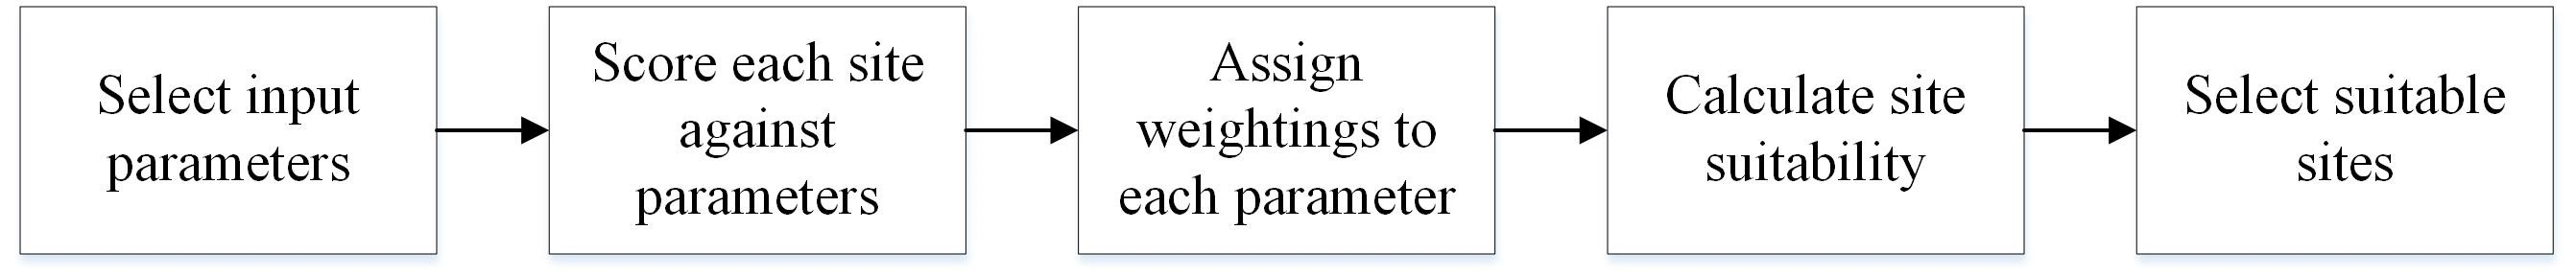
\includegraphics[width=1\linewidth]{figures/Stages} \caption{Typical stages of geospatial models for assessing wind turbine site suitability}\label{fig:StagesofAnalysis}
\end{figure}

Similar parameters are used throughout the studies, and ideal sites are
typically identified as having high average wind speeds; not being close
to urban areas; not in protected landscapes (e.g.~National Parks); not
close to airports (to minimise radar interference); close to roads for
access and finally close to power lines for grid connection. However the
weights for each parameter in subsequent predictive models have
traditionally been determined using surveys and questionnaires (Baban
and Parry \protect\hyperlink{ref-Baban2001}{2001}, Aydin, Kentel, and
Duzgun (\protect\hyperlink{ref-Aydin2010}{2010}), Neufville
(\protect\hyperlink{ref-Neufville2013}{2013}), Atici et al.
(\protect\hyperlink{ref-Atici2015}{2015})) or previous literature (Gass
et al. \protect\hyperlink{ref-Gass2013}{2013}, Q. Wang, M'Ikiugu, and
Kinoshita (\protect\hyperlink{ref-Wang2014}{2014}), Watson and Hudson
(\protect\hyperlink{ref-Watson2015}{2015})). To the authors' knowledge,
there have been no attempts to statistically validate the relative
importance of parameters used and it is therefore unclear whether the
parameters currently used are actually appropriate for site approval
rates. In a significant contribution, this paper derives these weights
using a statistically rigorous methodology and then tests their ability
to correctly predict planning outcomes.

In addition, there is increased awareness of the wider social challenges
surrounding the development since geographical variables in themselves
are insufficient to explain patterns of implementation of wind power
(Toke, Breukers, and Wolsink \protect\hyperlink{ref-Toke2008}{2008},
Devine-Wright (\protect\hyperlink{ref-Devine-Wright2005a}{2005})).
Recent studies have explored how planning decisions were influenced by
key actors (e.g.~local communities, planning authorities, project
developers) (Toke, Breukers, and Wolsink
\protect\hyperlink{ref-Toke2008}{2008}, Haggett and Toke
(\protect\hyperlink{ref-Haggett2006}{2006})) and local characteristics
(Horst and Toke \protect\hyperlink{ref-VanderHorst2010}{2010}). In
particular, a study by Van Rensburg et al. (Rensburg, Kelley, and
Jeserich \protect\hyperlink{ref-VanRensburg20}{2015}) explored wind
farms project planning approval against a range of technological and
institutional process variables. The results suggested a number of
variables appeared significant for planning including the proximity to
Natura 2000 sites (an EU protected habitat designation); sites with high
bird sensitivity; hub height and project installed capacity. In
addition, the study noted that proximity of the nearest dwellings and
wind speeds appeared insignificant, a finding which counters the views
reported within many previous studies. Other work has investigated the
social factors that may influence planning decisions (Langer et al.
\protect\hyperlink{ref-Langer2016a}{2016}, Álvarez-Farizo and Hanley
(\protect\hyperlink{ref-Alvarez-Farizo2002}{2002}), P. A. Groothuis,
Groothuis, and Whitehead (\protect\hyperlink{ref-Groothuis2008}{2008}),
Krueger, Parsons, and Firestone
(\protect\hyperlink{ref-Krueger2011}{2011}), Jones and Richard Eiser
(\protect\hyperlink{ref-Jones2010a}{2010})). For example, studies within
Great Britain suggest that support for wind developments decreases as
both income and age increase {[}31{]}, and people with higher levels of
qualifications are less likely to support projects (Krueger, Parsons,
and Firestone \protect\hyperlink{ref-Krueger2011}{2011}). However,
whilst these potential social factors have been identified, there have
been no attempts to include these parameters within geospatial analysis
of potential turbine developments. This work therefore integrates the
demographic and political parameters into geospatial analysis with the
aim of improving the validity of such a model.

In consequence this paper builds upon many of the concepts developed by
Van Rensburg et al., but aims to apply these concepts to a broader range
of geospatial, demographic and political datasets.

\section{Data and Variables}\label{data-and-variables}

An extensive literature review was conducted to identify geospatial and
social parameters which have been connected to the planning outcomes of
wind turbine applications. Parameters were collated from existing
geospatial models, and reviewing qualitative and quantitative studies.
The key sources included Baban and Parry (Baban and Parry
\protect\hyperlink{ref-Baban2001}{2001}), Langer et al. (Langer et al.
\protect\hyperlink{ref-Langer2016a}{2016}) and European Wind Energy
Association (European Wind Energy Association
\protect\hyperlink{ref-EuropeanWindEnergyAssociation2012}{2012}).

\subsection{Study Region}\label{study-region}

The study was conducted across Great Britain (England, Scotland \&
Wales). This was chosen because of the broadly similar categorisation of
land types, nature designation, data availability and legislation across
these regions.

\subsection{Data Sources}\label{data-sources}

Information for turbine planning applications was collected through the
Renewable Energy Planning Database (REPD) (DECC
\protect\hyperlink{ref-DECC2016}{2016}) with planning dates between
January 1991 and December 2016 (n=1755). Detailed information for each
planning application includes the location; year of application; number
of turbines; turbine capacity and planning decision.

The planning permission status was summarised to two variables: accepted
and rejected. Figure \ref{fig:StudyExtent} highlights the location of
the sites the distribution of these points and the planning status.

\begin{figure}
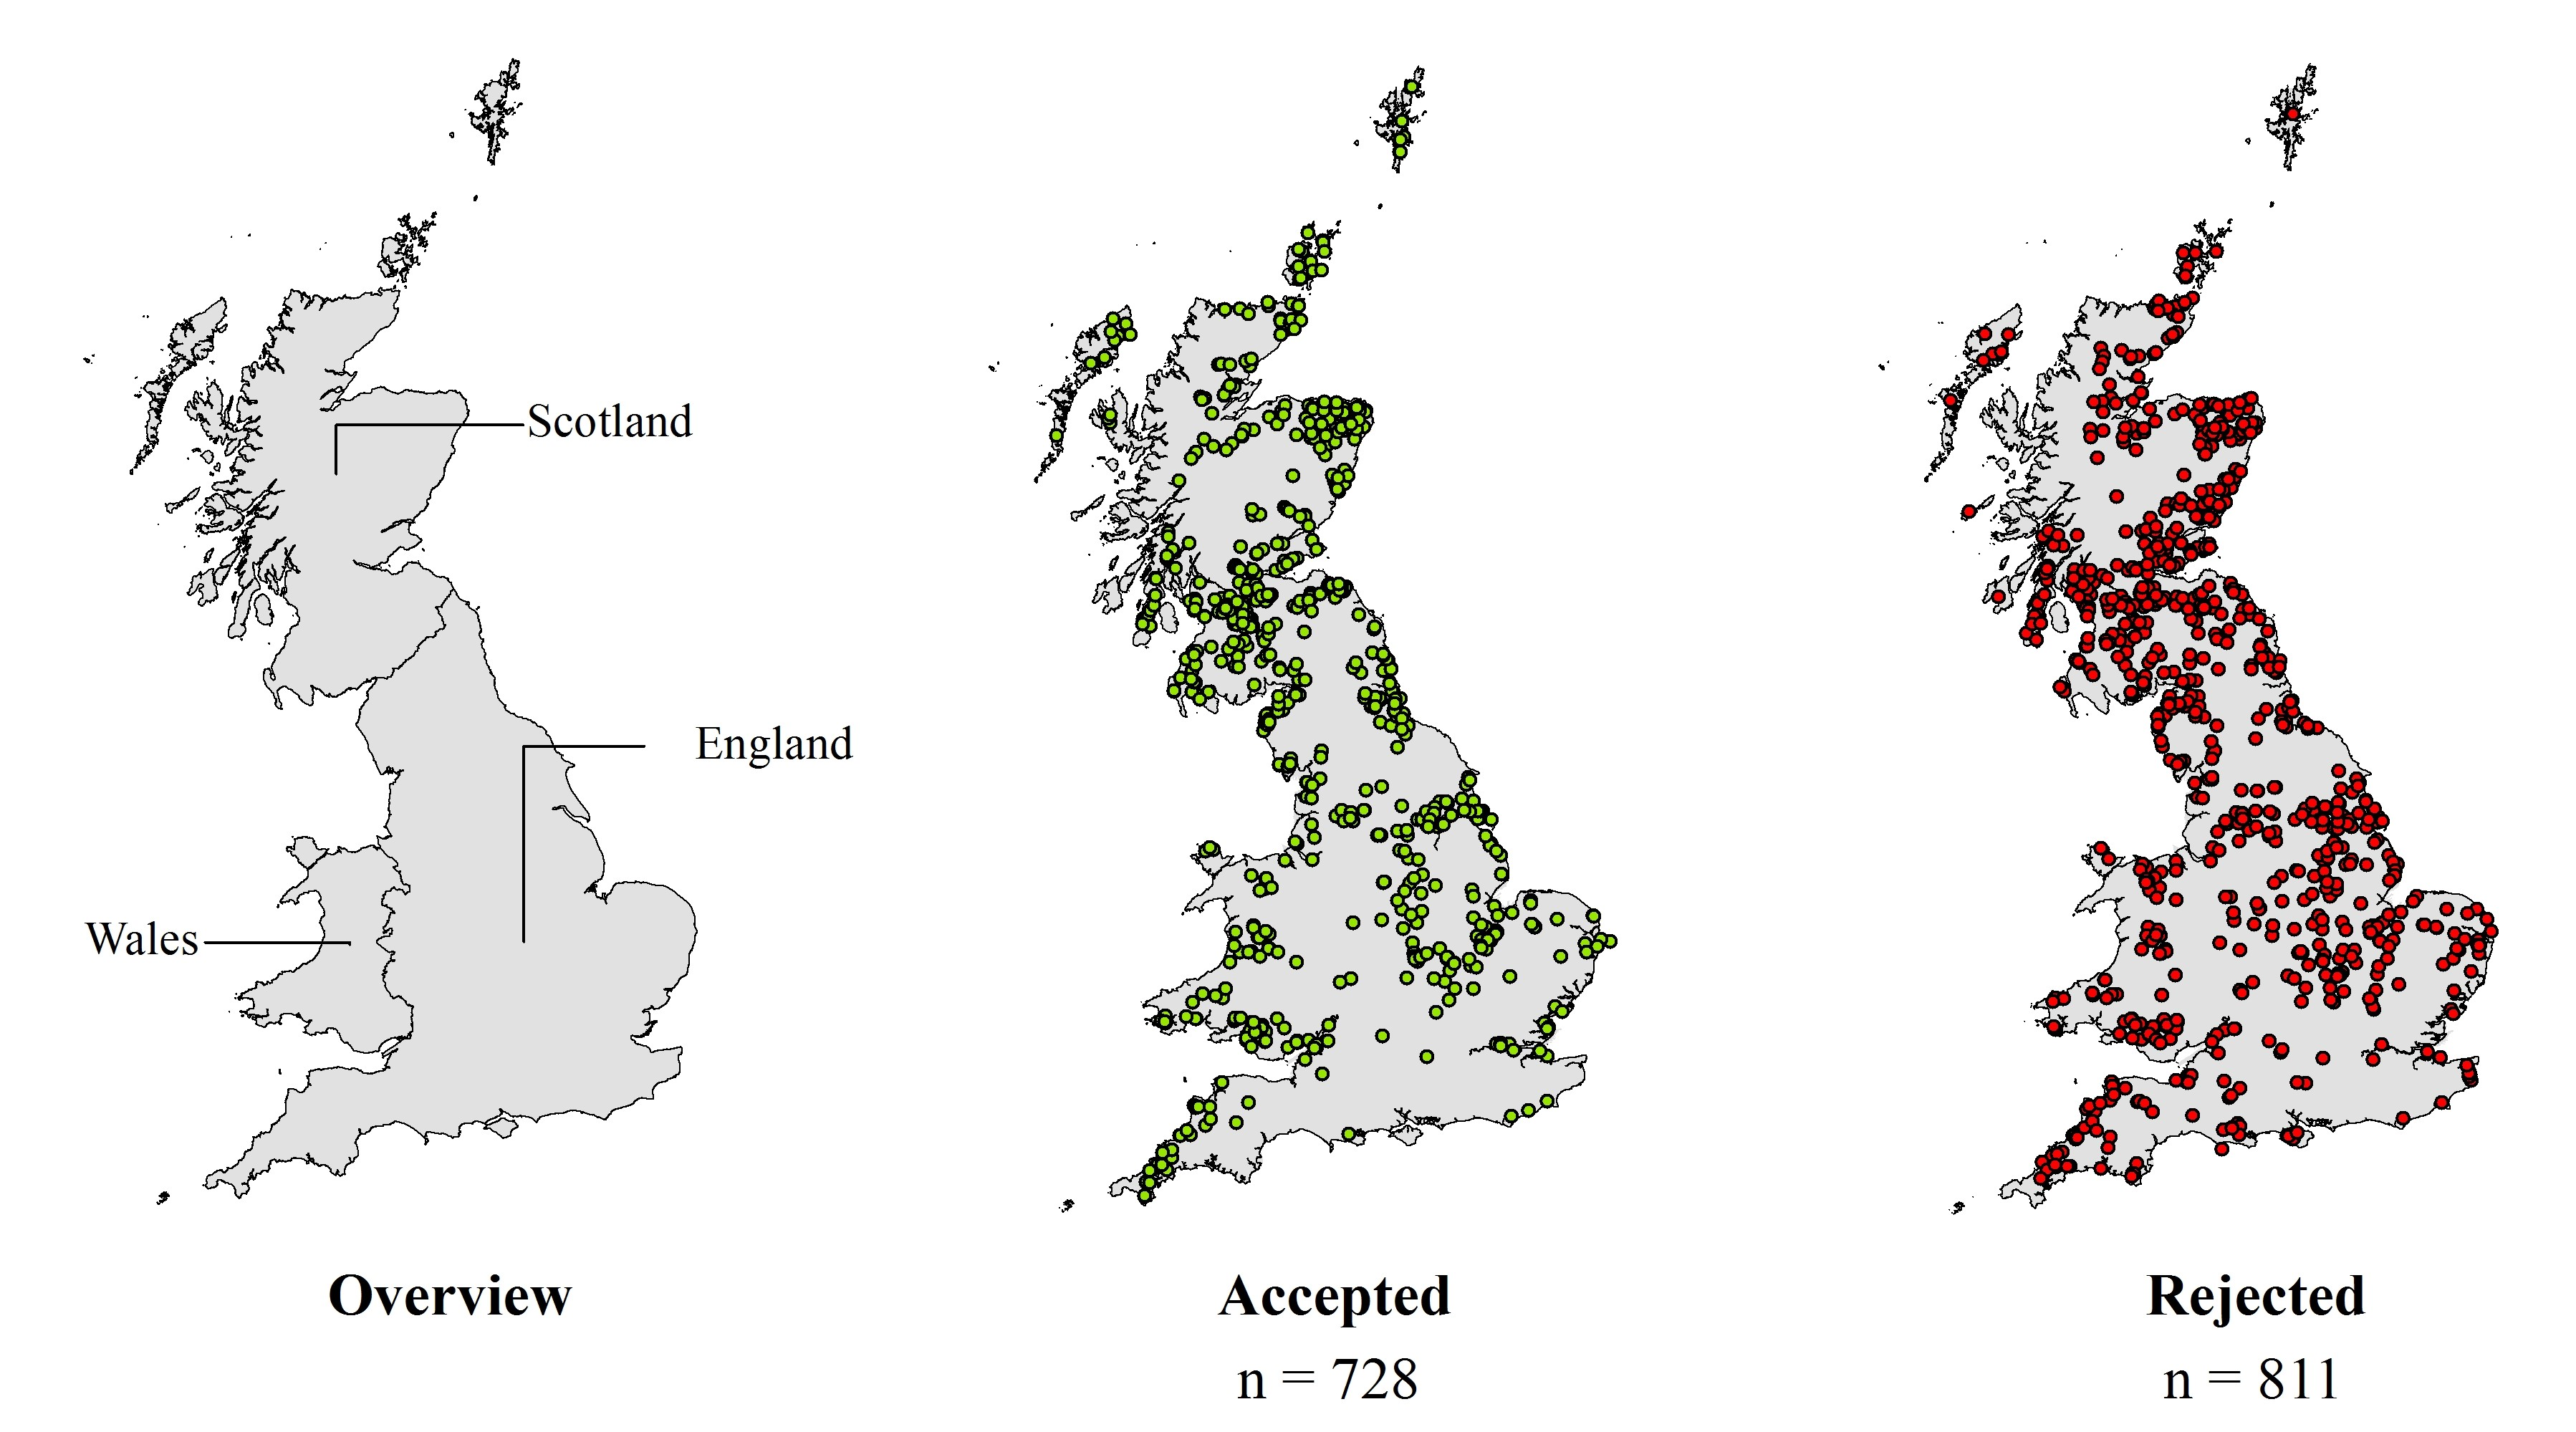
\includegraphics[width=1\linewidth]{figures/StudyExtent} \caption{Location of onshore wind turbine planning applications used within the study. Location data extracted from the Renewable Energy Planning Database}\label{fig:StudyExtent}
\end{figure}

Wind speeds were taken from the Numerical Objective Analysis of Boundary
Layer (NOABL) wind speed database, which provides estimated annualised
wind speed at 45m elevation at a resolution of 1km grid (DTI
\protect\hyperlink{ref-DTI2001}{2001}). This source is used extensively
by wind assessment studies conducted within the UK {[}4, 10, 17{]}.
Physical features including roads, railways and urban areas were
collected from OS Strategi (Ordnance Survey
\protect\hyperlink{ref-Survey2016}{2016}). The electricity transmission
network and Airport location data (civil and military) were extracted
from Open Street Maps (OSM) (OSM
\protect\hyperlink{ref-Overpass2016}{2016}).

Site elevation and slope is used by a number of studies to determine
site suitability (Baban and Parry
\protect\hyperlink{ref-Baban2001}{2001}, Janke
(\protect\hyperlink{ref-Janke2010}{2010})). Elevation was extracted from
a Digital Elevation Model (DEM) of Europe at a 25m resolution (EEA
\protect\hyperlink{ref-EEA2013}{2013}). This data was then used to
calculate the slope using the slope calculation tool within ArcGIS 10.2.

Census data was collected at the Lower Super Output Area (LSOA) and Data
Zone (Scotland) which represents regions with a population between 1000
and 3000 people. Data was collected for mean age; social grade
(percentage of higher social class AB, representing higher \&
intermediate managerial, administrative, professional occupations);
tenure (ownership of homes) and levels of qualifications (percentage of
population with university degree).

Planning decisions for turbines are influenced by the Local Planning
Authority, which are the local political bodies within the UK (HM
Government \protect\hyperlink{ref-HMGovernment2014}{2014}). In total,
there are 405 local authorities across England, Scotland and Wales. Data
was collected for the Conservatives; Labour, Liberal Democrat and the
Scottish National Party (SNP), which between them hold 95\% of seats
within Great Britain.

\subsection{Data Transformations}\label{data-transformations}

The data sources came in a range of formats including points, lines and
polygons (roads, urban regions etc.), tabular (census and political
data) and rasters (wind speed, elevation, slope) as highlighted in
Figure \ref{fig:MappingParameters}. These parameters had to be
summarised for each wind turbine farms within the model. ArcGIS 10.3 was
used to aggregate the datasets as follows:

\begin{itemize}
\tightlist
\item
  \textbf{Points, lines and polygons}: A spatial join was completed to
  find the distance to the nearest feature for each turbine. A value of
  0 is given if the turbine is within the feature.
\item
  \textbf{Tabular}: corresponding political and census boundaries were
  used to map the tabular data, and turbines assigned the value of the
  region. In addition, political data was filtered to the year of the
  planning application to determine the political balance at the time of
  planning.
\item
  \textbf{Raster}: The tool ``Raster Value to Point'' was used to
  extract the values for each site. The complete list of parameters used
  within the analysis is shown in Appendix A.
\end{itemize}

\begin{figure}
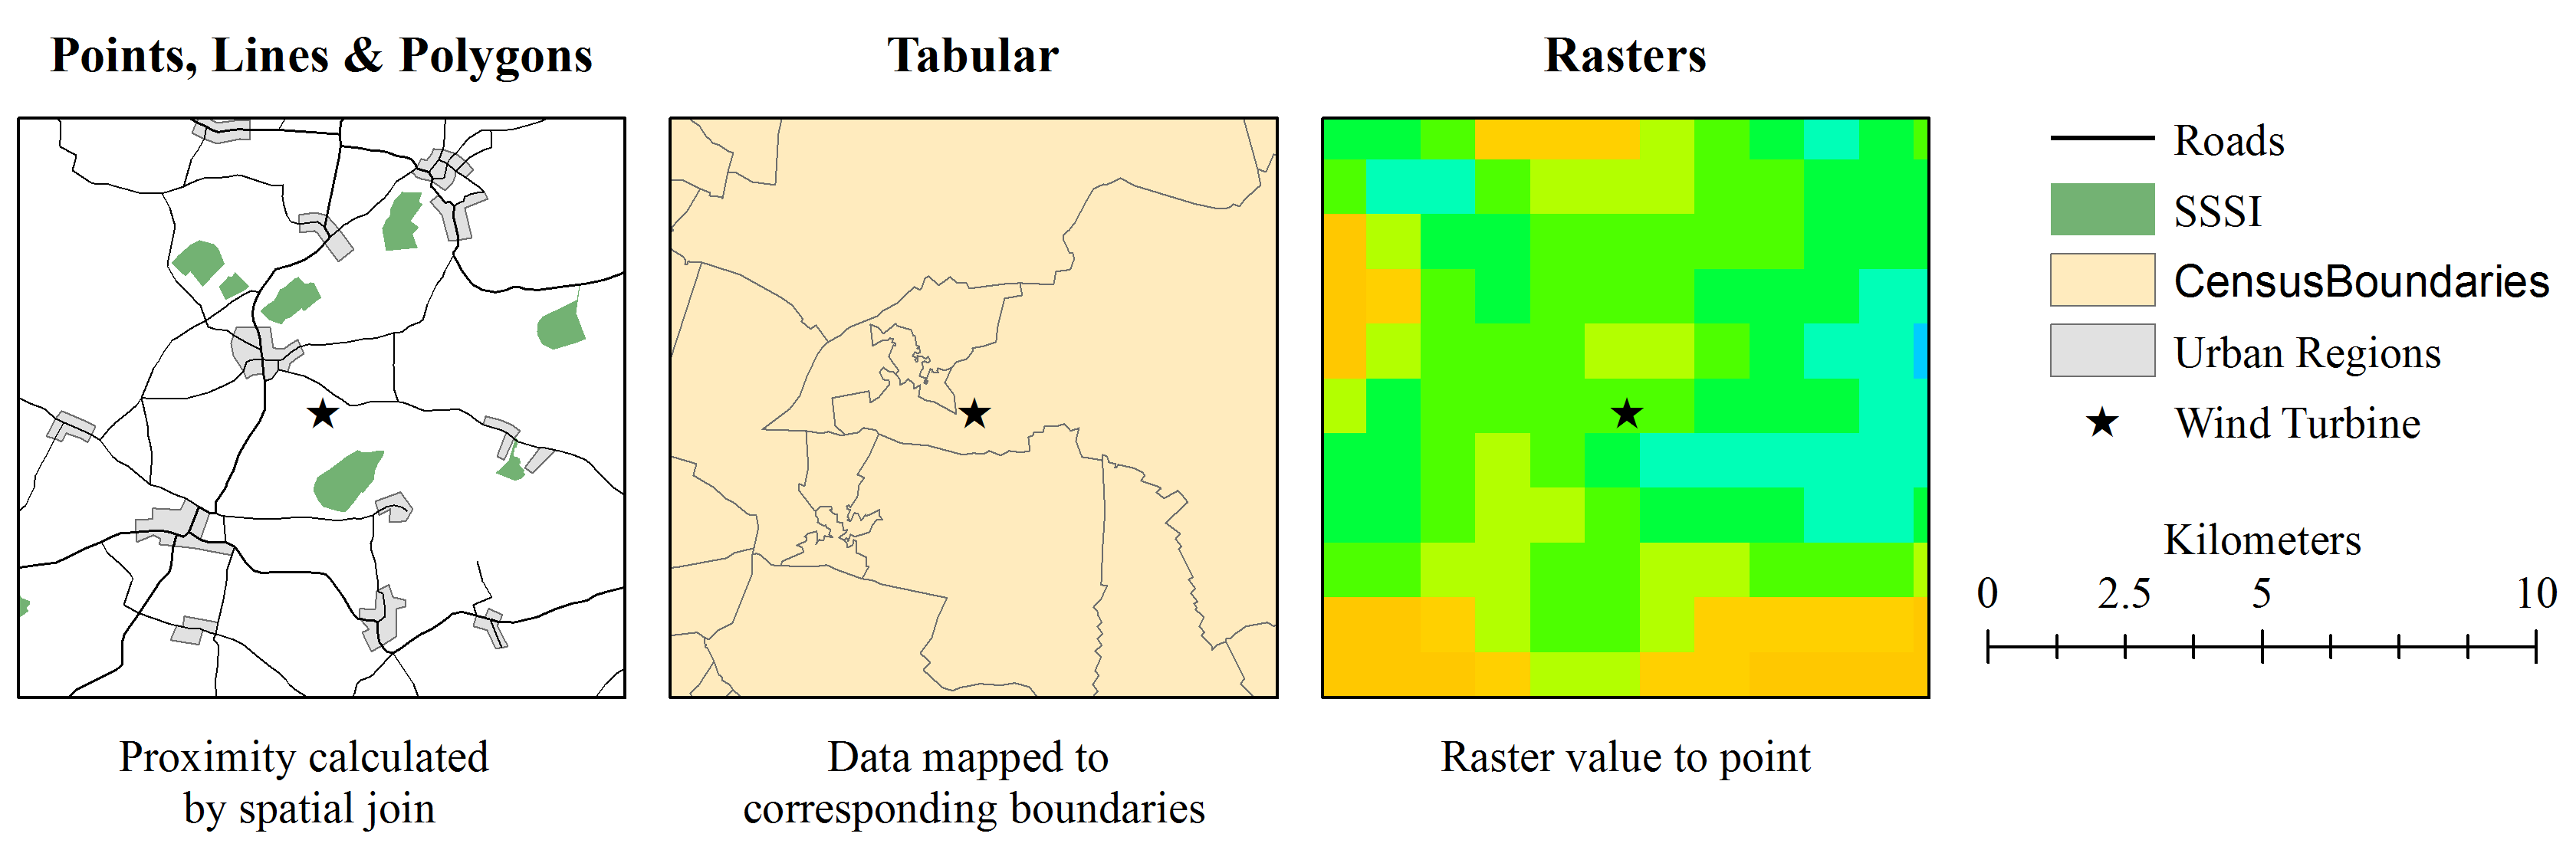
\includegraphics[width=1\linewidth]{figures/MappingParameters} \caption{Mapping of Parameter data to turbine locations}\label{fig:MappingParameters}
\end{figure}

\section{Methodology}\label{methodology}

A logistic regression analysis was conducted to model the factors
associated with a positive planning outcome of wind turbine applications
using the predictor variables listed in Table \ref{tab:ModelsSummary}. A
hierarchical approach was applied to the model building by adding
variables sequentially based on the following order of priority:
Physical attributes of the site; Distance to Features; Environmental and
Natural Designations; Social (Census) Data and finally Political Data.
This order was selected to reflect the current approach of geospatial
studies, which as mentioned above, generally do not consider the last
two.

For each additional set of parameters added to the model, diagnostic
checks were made to ensure that the assumptions of logistic regression
were maintained. Each parameter was checked for linearity of the logit
for independent variables, absence of multicollinearity and independence
of variables (Harrell \protect\hyperlink{ref-Harrell2001}{2001}). Any
parameters which violated these conditions were removed from the model.
The overall fit of the model was assessed using Pearson chi-squared,
Psuedo R2 values and the residual deviance. Internal validation was used
to assess the predictive accuracy of the model (Hosmer and Lemeshow
\protect\hyperlink{ref-Hosmer2004}{2004}).

Once all parameters had been included within the model, a parsimonious
model (one that accomplishes a desired level of explanation or
prediction with as few predictor variables as possible) was produced to
remove uninfluential parameters {[}44{]}. The Akaike Information
Criterion (AIC) was used to determine the best fitting subset of
parameters. This method avoids the issues associated with step-wise
approaches of parameter removal (Harrell
\protect\hyperlink{ref-Harrell2001}{2001}) and resulted in nine
effective parameters.

In addition, regional differences in parameters effects between England,
Scotland and Wales were hypothesised due to differing population
densities (England: 413/km\textsuperscript{2}, Wales:
149/km\textsuperscript{2}, Scotland: 68/km\textsuperscript{2}) (ONS
\protect\hyperlink{ref-ONS2013}{2013}) as well as differing
institutional support, with Scotland in particular placing a greater
emphasis on the development of onshore wind {[}46{]}. To test this,
separate logistic regression models were produced for each country.
These re-used the subset of influential nine parameters (see Figure
\ref{fig:OddsPlotSegmented}) with the additional inclusion of Wind
Speed, which had been suggested to be influential in previous research
(Rensburg, Kelley, and Jeserich
\protect\hyperlink{ref-VanRensburg20}{2015}).

\section{Results}\label{results}

Table \ref{tab:LogisticResults} provides the results from the
parsimonious logistic regression analysis associating planning approval
for all available cases. Statistically significant positive trends
(e.g.~increase in the parameter increases success rates) were observed
for Number of Turbine; Distance to Urban Regions; Distance to National
Parks; Percentage of local council Liberal Democrat and Percentage of
local council Labour. Negative associations were found for
Qualifications above L4 (university degree); Mean Age and Distance to
Natura 2000 sites. The odds ratios (OR) are shown for each parameter in
Figure 4, whereby an OR = 1 means the parameter does not affect odds of
the planning outcome, OR \textgreater{} 1 indicate the parameters
positively influence planning acceptance, OR \textless{} 1 represents a
negative parameter influence.

As noted, the reduced parameter set of parameters were also used to
assess models for England, Scotland and Wales separately and the odds
ratios for each parameter for these models are shown in Figure
\ref{OddsPlotSegmented}.

Finally, a summary of the different logistic models is shown in Table
\ref{tab:ModelsSummary}.

\begin{table}

\caption{\label{tab:LogisticResults}Logistic Regression results for the AIC optimised model.}
\centering
\begin{tabular}[t]{lrrrlrrr}
\toprule
Variable & Estimate & Std. Error & Pr & Sig. & Odds Ratio & 2.50\% & 97.50\%\\
\midrule
(Intercept) & 1.675 & 0.755 & 0.027 & * & 5.337 & 1.220 & 23.596\\
Number of Turbines & 0.017 & 0.007 & 0.010 & ** & 1.018 & 1.005 & 1.032\\
Distance to  Urban Region & 0.158 & 0.051 & 0.002 & ** & 1.171 & 1.060 & 1.295\\
Distance to National Park & 0.008 & 0.002 & 0.000 & *** & 1.008 & 1.005 & 1.011\\
Distance to Ramsar & 0.007 & 0.004 & 0.089 & . & 1.007 & 0.999 & 1.014\\
\addlinespace
Distance to SPA & -0.013 & 0.006 & 0.041 & * & 0.987 & 0.974 & 0.999\\
Qualifications, L4 & -0.036 & 0.007 & 0.000 & *** & 0.965 & 0.952 & 0.978\\
Mean Age & -0.043 & 0.016 & 0.006 & ** & 0.958 & 0.928 & 0.988\\
Political, Labour Share & 0.009 & 0.003 & 0.001 & *** & 1.009 & 1.004 & 1.015\\
Political, Liberal Democrat & 0.009 & 0.004 & 0.030 & * & 1.009 & 1.001 & 1.017\\
\bottomrule
\end{tabular}
\end{table}

\begin{table}

\caption{\label{tab:ModelsSummary}A summary of the logistic regression models}
\centering
\begin{tabular}[t]{llllll}
\toprule
Variable & Full & Reduced & Nested:
England & Nested:
Scotland & Nested:
Wales\\
\midrule
Observations & 1476 & 1476 & 646 & 698 & 132\\
Parameters & 27 & 9 & 10 & 11 & 10\\
Nagelkirke R2 & 0.11 & 0.1 & 0.11 & 0.16 & 0.24\\
Pearson Chi-squared & 113.7 & 111.9 & 51.5 & 89.3 & 25.9\\
Residual deviance & 1932 & 1932 & 833 & 895 & 157\\
Model Accuracy & 60\% & 62\% & 60\% & 65\% & 57\%\\
\bottomrule
\end{tabular}
\end{table}

\begin{figure}
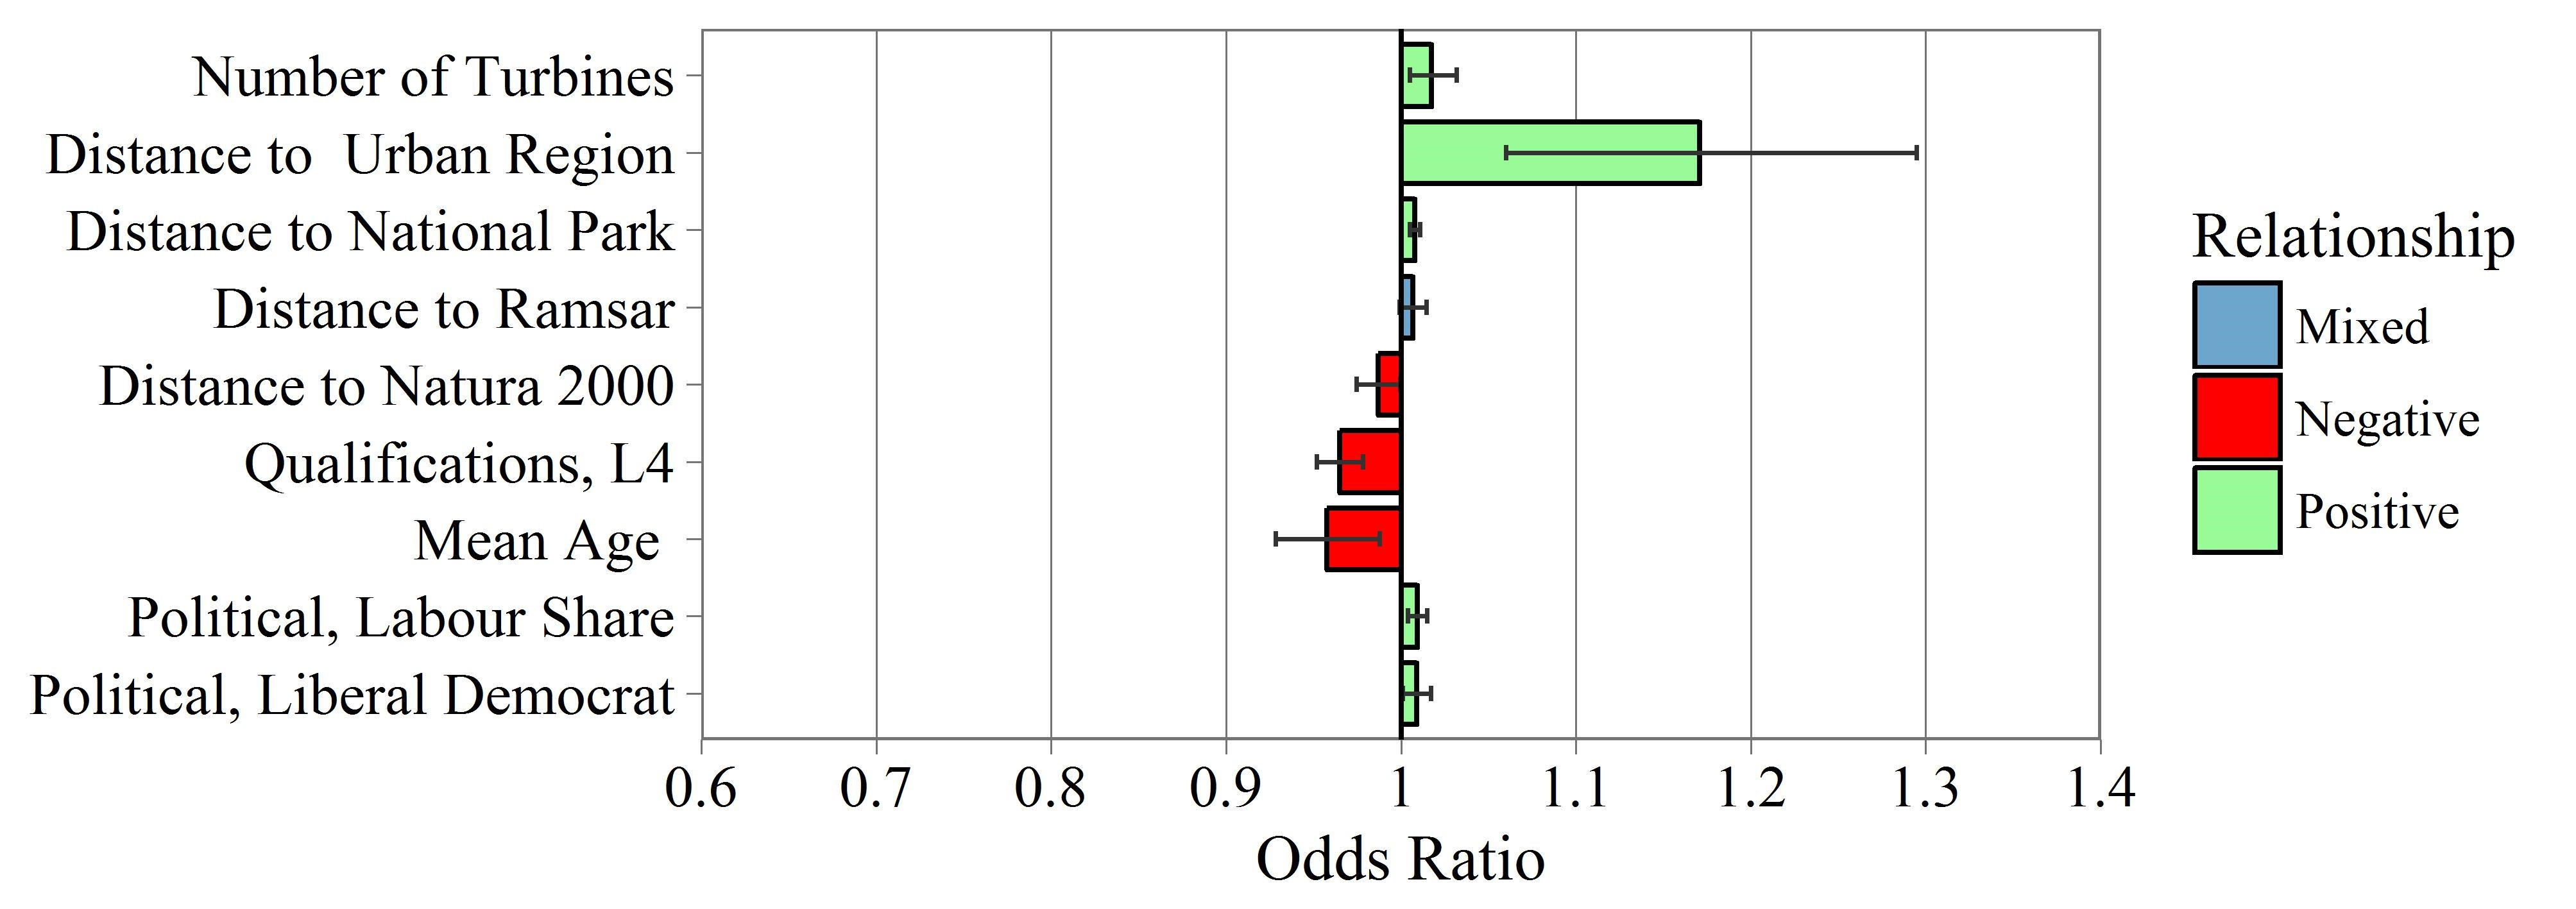
\includegraphics[width=1\linewidth]{figures/OddsPlotReduced} \caption{Odds plot for the reduced logistic regression mode. Error bars show the 95 confidence interval.}\label{fig:OddsPlotReduced}
\end{figure}

\begin{figure}
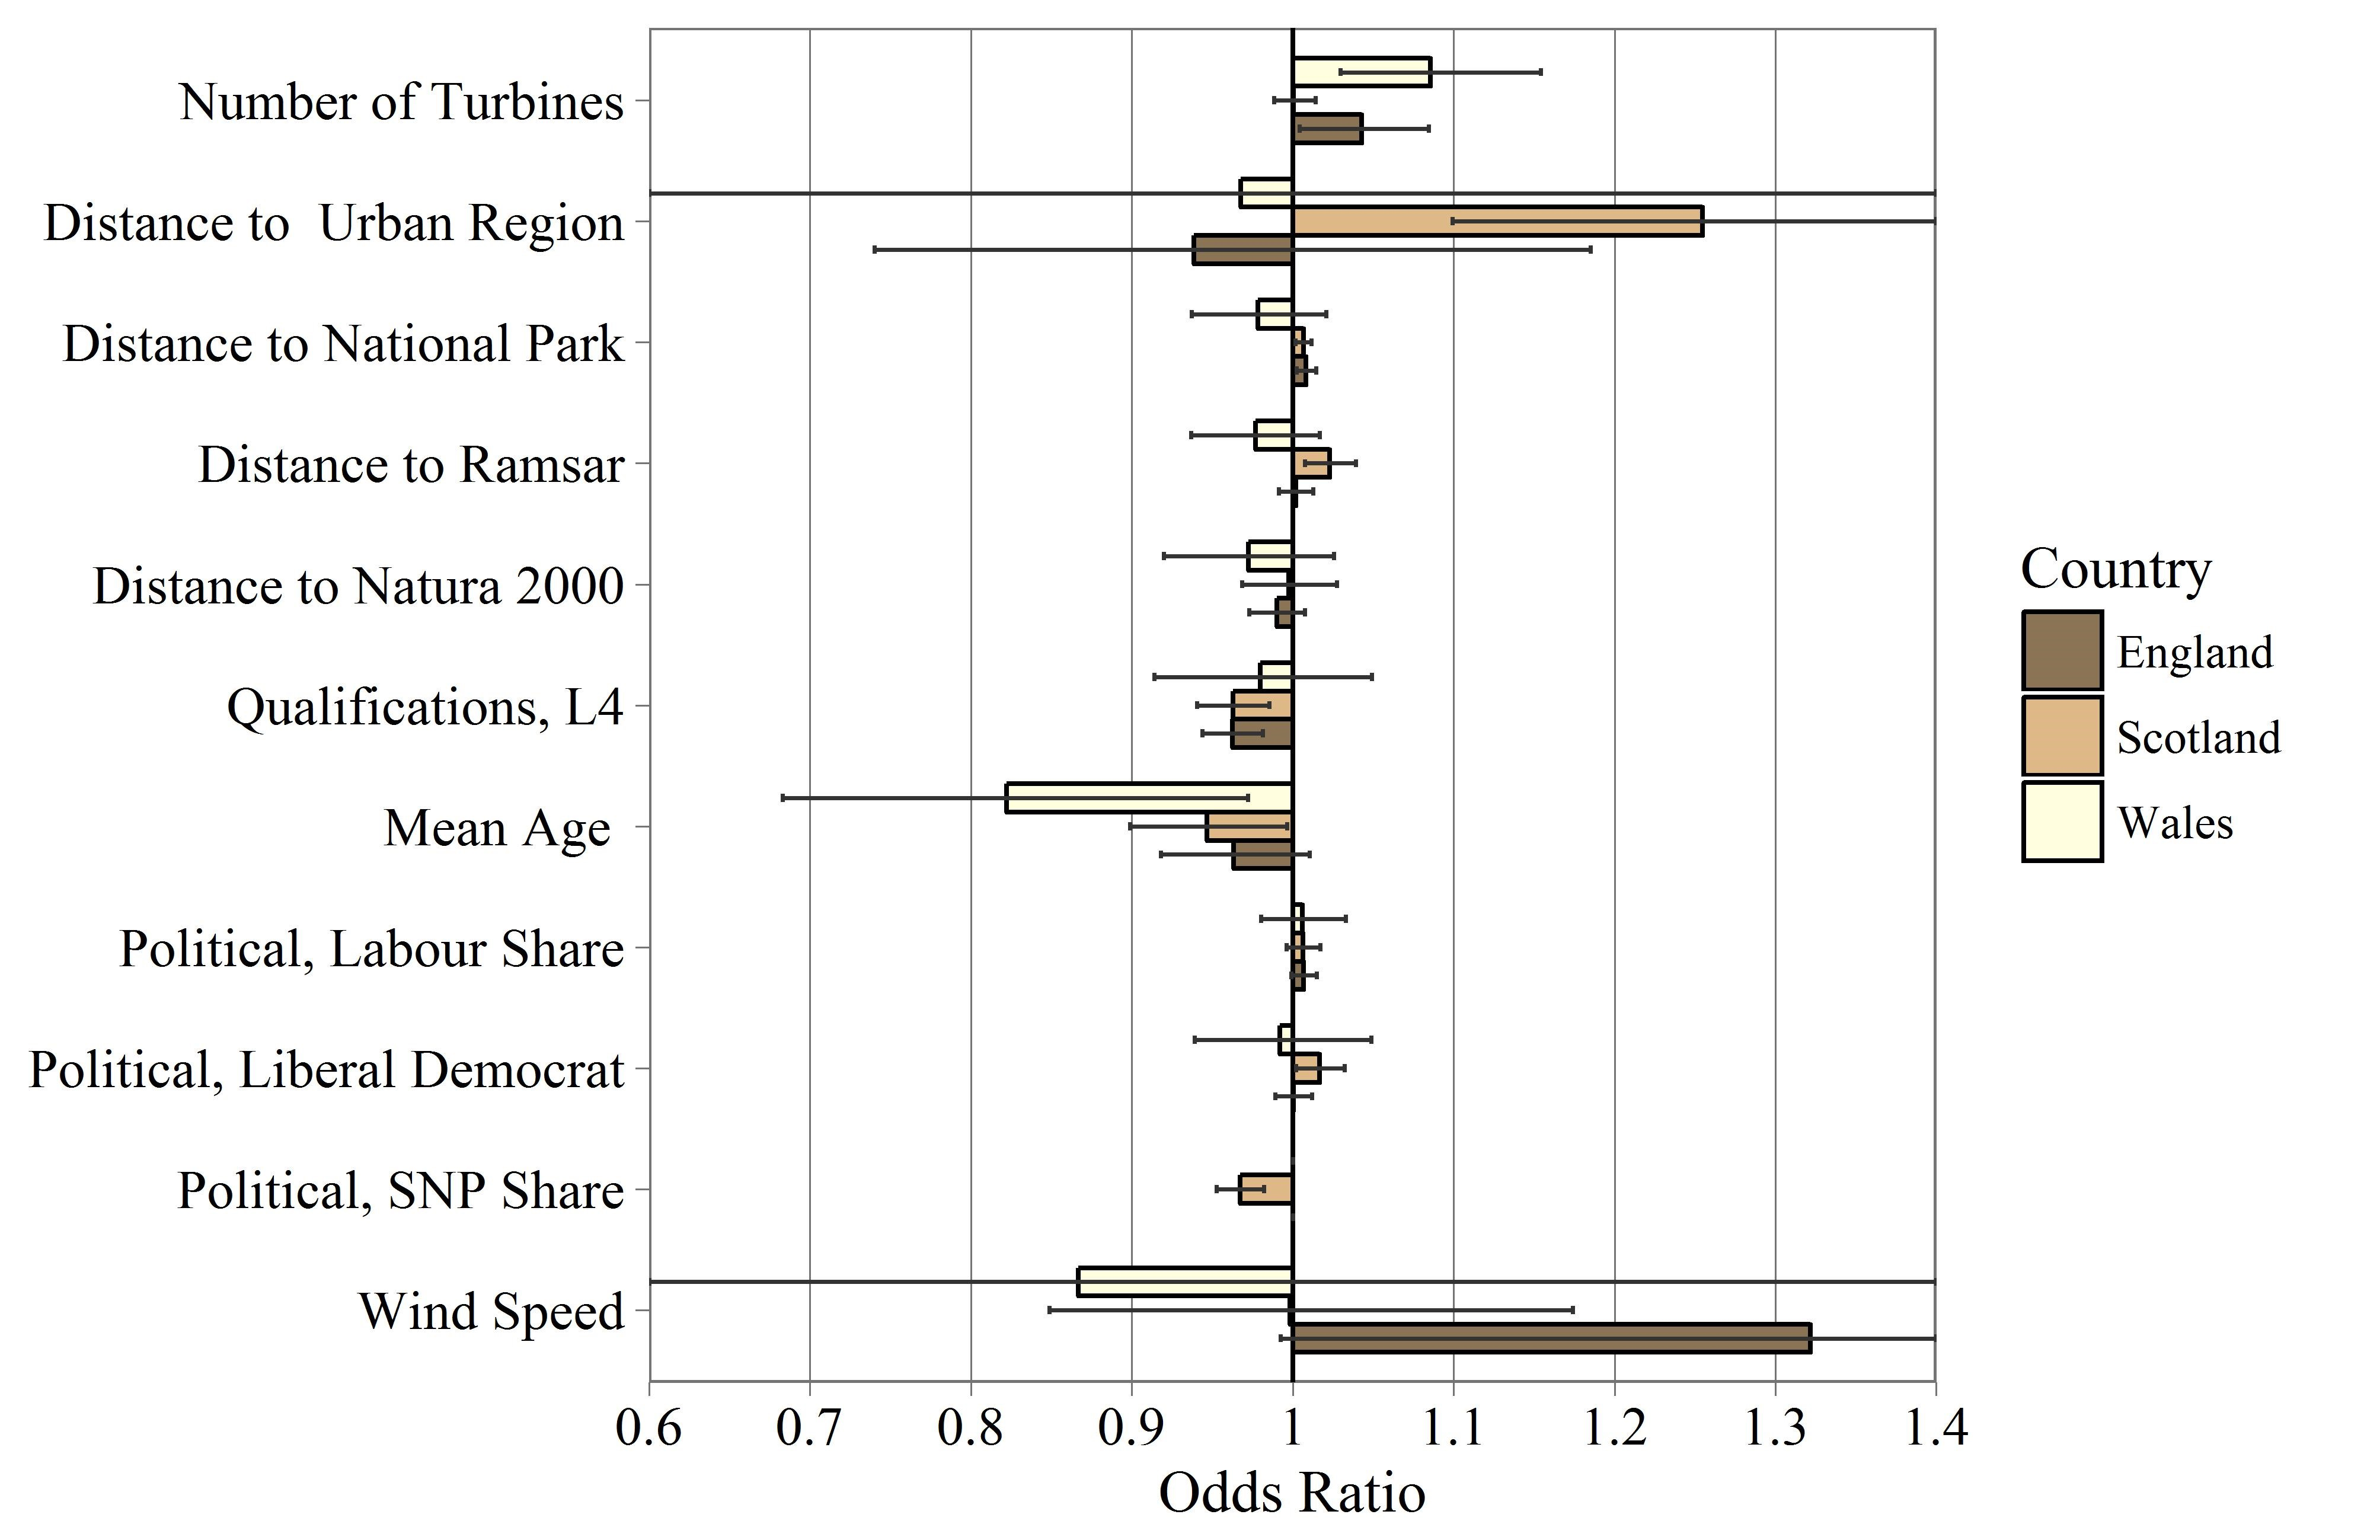
\includegraphics[width=1\linewidth]{figures/OddsPlotSegmented} \caption{Odds plot for the nested logistic regression models for England, Scotland and Wales. Error bars indicate 95 confidence intervals.}\label{fig:OddsPlotSegmented}
\end{figure}

\section{Discussion}\label{discussion}

The ``all countries'' model highlighted several key parameters, as shown
in Figure \ref{OddsPlotReduced}. First, for project characteristics, the
number of turbines appears significant in determining project success
although the magnitude of the effect is relatively small. It is
suggested that developers are more likely to appeal the decisions made
against larger wind farms, as rejection of such projects would result in
a large loss of revenue.

A number of physical parameters have been identified as significant. The
distance to urban areas has been highlighted as an indicator, although
with considerable uncertainty as the confidence intervals indicate.
There are a number of potential causes for this: firstly, it could
indicate that high wind speed sites suitable for development tend to be
naturally less populated (i.e.~hilly, isolated regions). Additionally,
it may reflect a so-called ``Not in My Back Yard'' (NIMBY) view from
local population, with project in closer proximity to urban areas being
more likely to be rejected. However, there are conflicting views in
literature whether NIMBY views impact wind turbines, with a range of
positive (Haggett and Toke \protect\hyperlink{ref-Haggett2006}{2006},
Jones and Richard Eiser (\protect\hyperlink{ref-Jones2010a}{2010})) and
negative (Rensburg, Kelley, and Jeserich
\protect\hyperlink{ref-VanRensburg20}{2015}, Devine-Wright
(\protect\hyperlink{ref-Devine-Wright2005a}{2005}), Populus
(\protect\hyperlink{ref-Populus2005}{2005})) studies.

For Landscape and environmental designations, distance to National Parks
and Natura 2000 sites were indicated as significant, although have
marginal impacts. It had been expected that such parameters would be
more influential, as the visual impact of wind turbine land is often
stated as a reason for project refusal (Jones and Richard Eiser
\protect\hyperlink{ref-Jones2010a}{2010}).

Both the level of qualifications, and the mean age of the local populous
have been retained as significant parameters for Demographic variables.
It is suggested that regions of higher education may be more effective
in organising campaign groups against such projects. This supports the
hypothesis developed by Van der Horst and Toke (Horst and Toke
\protect\hyperlink{ref-VanderHorst2010}{2010}) that developers were
``keen to avoid relatively privileged communities and target areas where
people are thought to less likely put up a fight''.

For political variables, the percentage of local council authority
control for Liberal Democrats and Labour both appear significant. It is
suggested that this may be because these parties are broadly supportive
of wind projects at a national level, and as such, local planning
decisions may be more favourable for proposed projects. In addition,
other studies have highlighted that voters of these parties are
personally more in favour of onshore wind (Populus
\protect\hyperlink{ref-Populus2005}{2005}), which may result in less
local objection against projects in areas where they have stronger
support.

There are notable parameters which do not prove influential, including
wind speed and the proximity to airports. This may reflect that these
parameters represent technical challenges which can be investigated in
the early stages of project development, and therefore any sites that
are not suitable will not seek planning permission.

Figure 5 highlights that, as hypothesised, the odds ratios for
parameters vary by country, although the reduced number of cases in each
model increases the uncertainty substantially as indicated by the
confidence intervals. It can be seen that parameters such as Turbine
Capacity; Wind Speed and Distance to Urban Regions show differing
relationships for each country. These suggest that there may be
differing motives for projects within each country as well as
differential planning constraints. For example, projects within England
appear to place higher emphasis on wind speed. It should be noted that
the wind resource is more marginal in England, and it is suggested that
low wind speed may be an easy way for projects to be rejected.

For the Scotland model, the percentage of local council authority
control for SNP appears significant, with increased percentage resulting
in a lower acceptance rate. However, upon further inspection, this was
deemed to be a potential confounding variable with the year of
application: SNP have increased their share of council seats between
1990 and 2016 from 15\% to 35\%, while at the same time the average
acceptance rates have reduced from around 75\% to 40\% across that
period. This parameter therefore appears to capture a national trend,
rather than highlighting any local political influences.

As shown in Table 3, there is a relatively low level of fit with Psuedo
R2 values of 0.1. Splitting the model into England, Scotland and Wales
marginally improved these values to 0.11, 0.16 and 0.24, suggesting the
model was a better fit for Scotland and Wales. However, while the
accuracy of the Scotland model improved against the ``all countries''
model (60\% to 65\%), the Wales only model has decreased to 57\%,
suggesting that this model has been overfitted due to the reduced number
of observations (n = 132).

\section{Conclusions \& Implications}\label{conclusions-implications}

This paper has investigated the influence of geospatial, environmental,
demographic and political attributes on the probability of wind farm
planning approval in Great Britain between 1990 and 2016. The study
findings reveal that local demographic and political parameters appear
to influence the planning outcomes of projects, and that many of the
geospatial parameters typically integrated into wind turbine models
appear insignificant in determining site approval. To the authors'
knowledge, such quantitative findings have not previously been
demonstrated using such datasets.

It appears that certain demographics are less accepting of onshore wind
in Great Britain. Given that UK planning policy has now devolved power
locally and allowing local communities to have the final say on projects
{[}48{]}, there may be a clear block to development in certain regions
in the country.

In addition, the results raise concerns of the predictive ability of
existing geospatial modelling in locating wind turbine sites. These
findings provide evidence to support existing literature that GIS tools
in themselves are of limited applicability (D. Toke
\protect\hyperlink{ref-Toke2005}{2005}, Malczewski
(\protect\hyperlink{ref-Malczewski2004}{2004})), and supports the
conclusion that greater emphasis needs to be given to the non-physical
elements of a project (e.g.~Community engagement with the scheme from an
early stage) (Toke, Breukers, and Wolsink
\protect\hyperlink{ref-Toke2008}{2008}, Wolsink
(\protect\hyperlink{ref-Wolsink2000}{2000}), Warren and McFadyen
(\protect\hyperlink{ref-Warren2010}{2010})).

Because of the low model fit, future work aims to integrate more
detailed information about specific wind turbine sites. It has not been
possible to include detailed information of the project development
within the analysis. Studies have highlighted that the interaction of
developers with local communities are key indicators of positive
planning approval outcomes (D. Toke
\protect\hyperlink{ref-Toke2005}{2005}, Devine-Wright
(\protect\hyperlink{ref-Devine-Wright2005a}{2005}), Wustenhagen,
Wolsink, and Burer (\protect\hyperlink{ref-Wustenhagen2007}{2007})).

It should be noted that the parameters used to derive these findings are
obtained with context to Great Britain, and therefore may have limited
applicability internationally, and therefore should be applied with
caution outside of this region. There are opportunities to expand upon
this work by exploring the international context of the finding to widen
its applicability.

\subsection*{Acknowledgments}\label{acknowledgments}
\addcontentsline{toc}{subsection}{Acknowledgments}

This work is part of the activities of the Energy and Climate Change
Division and the Sustainable Energy Research Group at the University of
Southampton \url{www.energy.soton.ac.uk}. It is also supported by ESPRC
under grant EP/J017698/1, Transforming the Engineering of Cities to
Deliver Societal and Planetary Wellbeing and the Faculty of Engineering
and Environment at the University of Southampton.

\subsection*{Supplementary Files}\label{supplementary-files}
\addcontentsline{toc}{subsection}{Supplementary Files}

The supporting data and analysis is available on Southampton Eprints
\href{https://eprints.soton.ac.uk/408181/}{(https://eprints.soton.ac.uk/408181/)}
and through GitHub
\href{https://github.com/mikey-harper/WindStatisticalAnalysis}{(https://github.com/mikey-harper/WindStatisticalAnalysis)}

\begin{landscape}\begin{table}

\caption{\label{tab:unnamed-chunk-1}Summary of data sources used within model}
\centering
\resizebox{\linewidth}{!}{\begin{tabular}[t]{rlllllll}
\toprule
ID & Category & Variable & Source & Data Type & Variable Value & Value Type & Unit\\
\midrule
1 & Turbine & Wind Turbine Planning Data & REPD & Tabular & Planning Outcome & Categorical & Accept/Reject\\
2 &  & Turbine Capacity &  & Tabular & Megawatts/turbine & Continuous & MW\\
3 &  & Number of Turbines &  & Tabular &  & Continuous & \\
4 &  & Year &  & Tabular &  & Discrete & \\
5 &  & Country &  & Tabular &  & Categorical & \\
\addlinespace
6 & Resource & Wind Speed & NOABL & Raster & Annualised Wind Speed & Continuous & m/s\\
7 & Features & Airports & OpenGeo & Points & Distance to Feature & Continuous & km\\
8 &  & Roads * & OS Strategi & Lines & Distance to Feature & Continuous & km\\
9 &  & Railways &  & Lines & Distance to Feature & Continuous & km\\
10 &  & Urban Areas &  & Polygons & Distance to Feature & Continuous & km\\
\addlinespace
11 &  & HV Powerlines ** &  & Lines & Distance to Feature & Continuous & km\\
12 & Landscape & Areas of Outstanding Natural Beauty & National Heritage & Polygons & Distance to Feature & Continuous & km\\
13 &  & National Parks &  & Polygons & Distance to Feature & Continuous & km\\
14 &  & Heritage Coast &  & Polygons & Distance to Feature & Continuous & km\\
15 & Nature & Special Protection Areas &  & Polygons & Distance to Feature & Continuous & km\\
\addlinespace
16 &  & National Nature Reserve &  & Polygons & Distance to Feature & Continuous & km\\
17 &  & Sites of Special Scientific Interest &  & Polygons & Distance to Feature & Continuous & km\\
18 &  & Special Areas of Conservation &  & Polygons & Distance to Feature & Continuous & km\\
19 & Geographic & Elevation & EU DEM & Raster & Height above sea level & Integer & m\\
20 &  & Slope & Derived from 18 & Raster & Gradient & Continuous & \%\\
\addlinespace
21 & Census & Level of Qualification & ONS & Tabular & Higher than L4 *** & Continuous & \%\\
22 &  & Age &  & Tabular & Mean & Continuous & Years\\
23 &  & Social Grade &  & Tabular & Social Grade AB **** & Continuous & \%\\
24 &  & Tenure &  & Tabular & Home Ownership & Continuous & \%\\
25 & Political & Conservatives & Populus & Tabular & Percentage of Council & Continuous & \%\\
\addlinespace
26 &  & Labour &  & Tabular & Percentage of Council & Continuous & \%\\
27 &  & Liberal Democrat &  & Tabular & Percentage of Council & Continuous & \%\\
\bottomrule
\multicolumn{8}{l}{\textsuperscript{a} * Roads are broken into four main categories: Motorways, A Roads, B Roads and Minor Roads. ** High Voltage network at 140-400kV. *** L4}\\
\multicolumn{8}{l}{represents degree level or above. **** AB represents Higher \& intermediate managerial, administrative, professional occupation}\\
\end{tabular}}
\end{table}
\end{landscape}

\section*{References}\label{references}
\addcontentsline{toc}{section}{References}

\hypertarget{refs}{}
\hypertarget{ref-Atici2015}{}
Atici, Kazim Baris, Ahmet Bahadir Simsek, Aydin Ulucan, and Mustafa Umur
Tosun. 2015. ``A GIS-based Multiple Criteria Decision Analysis approach
for wind power plant site selection.'' \emph{Utilities Policy} 37.
Elsevier Ltd: 86--96.
doi:\href{https://doi.org/10.1016/j.jup.2015.06.001}{10.1016/j.jup.2015.06.001}.

\hypertarget{ref-Aydin2010}{}
Aydin, Nazli Yonca, Elcin Kentel, and Sebnem Duzgun. 2010. ``GIS-based
environmental assessment of wind energy systems for spatial planning: A
case study from Western Turkey.'' \emph{Renewable and Sustainable Energy
Reviews} 14 (1): 364--73.
doi:\href{https://doi.org/10.1016/j.rser.2009.07.023}{10.1016/j.rser.2009.07.023}.

\hypertarget{ref-Alvarez-Farizo2002}{}
Álvarez-Farizo, Begoa, and Nick Hanley. 2002. ``Using conjoint analysis
to quantify public preferences over the environmental impacts of wind
farms. An example from Spain.'' \emph{Energy Policy} 30 (2): 107--16.
doi:\href{https://doi.org/10.1016/S0301-4215(01)00063-5}{10.1016/S0301-4215(01)00063-5}.

\hypertarget{ref-Baban2001}{}
Baban, Serwan M J, and Tim Parry. 2001. ``Developing and applying a
GIS-assisted approach to locating wind farms in the UK.''
\emph{Renewable Energy} 24 (1): 59--71.
doi:\href{https://doi.org/10.1016/S0960-1481(00)00169-5}{10.1016/S0960-1481(00)00169-5}.

\hypertarget{ref-DECC2016}{}
DECC. 2016. ``Renewable Energy Planing Data.''
\url{https://www.gov.uk/government/collections/renewable-energy-planning-data}.

\hypertarget{ref-Devine-Wright2005a}{}
Devine-Wright, Patrick. 2005. ``Beyond NIMBYism: Towards an integrated
framework for understanding public perceptions of wind energy.''
\emph{Wind Energy} 8 (2): 125--39.
doi:\href{https://doi.org/10.1002/we.124}{10.1002/we.124}.

\hypertarget{ref-DTI2001}{}
DTI. 2001. ``NOABL Windspeed Database.'' \url{https://goo.gl/6BALyv}.

\hypertarget{ref-EEA2013}{}
EEA. 2013. ``Digital Elevation Model over Europe (EU-DEM).''
\href{http://www.eea.europa.eu/data-and-maps/data/eu-dem\%7B/\#\%7Dtab-european-data}{http://www.eea.europa.eu/data-and-maps/data/eu-dem\{\textbackslash{}\#\}tab-european-data}.

\hypertarget{ref-EuropeanWindEnergyAssociation2012}{}
European Wind Energy Association. 2012. \emph{Wind Energy - The Facts: A
Guide to the Technology, Economics and Future of Wind Power}. Routledge.

\hypertarget{ref-Gass2013}{}
Gass, Viktoria, Johannes Schmidt, Franziska Strauss, and Erwin Schmid.
2013. ``Assessing the economic wind power potential in Austria.''
\emph{Energy Policy} 53 (2013). Elsevier: 323--30.
doi:\href{https://doi.org/10.1016/j.enpol.2012.10.079}{10.1016/j.enpol.2012.10.079}.

\hypertarget{ref-Groothuis2008}{}
Groothuis, Peter A., Jana D Groothuis, and John C Whitehead. 2008.
``Green vs. green: Measuring the compensation required to site
electrical generation windmills in a viewshed.'' \emph{Energy Policy} 36
(4): 1545--50.
doi:\href{https://doi.org/10.1016/j.enpol.2008.01.018}{10.1016/j.enpol.2008.01.018}.

\hypertarget{ref-Haggett2006}{}
Haggett, Claire, and David Toke. 2006. ``Crossing the great divide-using
multi-method analysis to understand opposition to windfarms.''
\emph{Public Administration} 84 (1): 103--20.
doi:\href{https://doi.org/10.1111/j.0033-3298.2006.00495.x}{10.1111/j.0033-3298.2006.00495.x}.

\hypertarget{ref-Hansen2005}{}
Hansen, H. S. 2005. ``GIS-based Multi-Criteria Analysis of Wind Farm
Development.'' \emph{Proceedings of the 10th Scandinavian Research
Confrence on Geographical Information Scient}, 75--87.

\hypertarget{ref-Harrell2001}{}
Harrell, Frank E. 2001. \emph{Regression modeling strategies. With
applications to linear models, logistic regression, and survival
analysis}.
doi:\href{https://doi.org/10.1007/978-1-4757-3462-1}{10.1007/978-1-4757-3462-1}.

\hypertarget{ref-HMGovernment2014}{}
HM Government. 2014. ``Planning Portal Northern Ireland.''

\hypertarget{ref-VanderHorst2010}{}
Horst, Dan van der, and David Toke. 2010. ``Exploring the landscape of
wind farm developments; local area characteristics and planning process
outcomes in rural England.'' \emph{Land Use Policy} 27 (2): 214--21.
doi:\href{https://doi.org/10.1016/j.landusepol.2009.05.006}{10.1016/j.landusepol.2009.05.006}.

\hypertarget{ref-Hosmer2004}{}
Hosmer, David W, and Stanley Lemeshow. 2004. \emph{Applied Logistic
Regression Second Edition}.
doi:\href{https://doi.org/10.1002/0471722146}{10.1002/0471722146}.

\hypertarget{ref-Janke2010}{}
Janke, J. R. 2010. ``Multicriteria GIS modeling of wind and solar farms
in Colorado.'' \emph{Renewable Energy} 35: 2228--34.
\href{http://people.umass.edu/bethanyb/Janke,\%202010.pdf}{http://people.umass.edu/bethanyb/Janke, 2010.pdf}.

\hypertarget{ref-Jones2010a}{}
Jones, Christopher R., and J. Richard Eiser. 2010. ``Understanding
'local' opposition to wind development in the UK: How big is a
backyard?'' \emph{Energy Policy} 38 (6). Elsevier: 3106--17.
doi:\href{https://doi.org/10.1016/j.enpol.2010.01.051}{10.1016/j.enpol.2010.01.051}.

\hypertarget{ref-Krueger2011}{}
Krueger, Andrew D., George R. Parsons, and Jeremy Firestone. 2011.
``Valuing the visual disamenity of offshore wind power projects at
varying distances from the shore: An application on the Delaware
shoreline.'' \emph{Land Economics} 87 (2): 268--83.
\href{http://www.scopus.com/inward/record.url?eid=2-s2.0-79951908702\%7B/\&\%7DpartnerID=tZOtx3y1}{http://www.scopus.com/inward/record.url?eid=2-s2.0-79951908702\{\textbackslash{}\&\}partnerID=tZOtx3y1}.

\hypertarget{ref-Langer2016a}{}
Langer, Katharina, Thomas Decker, Jutta Roosen, and Klaus Menrad. 2016.
``A qualitative analysis to understand the acceptance of wind energy in
Bavaria.'' \emph{Renewable and Sustainable Energy Reviews} 64. Elsevier:
248--59.
doi:\href{https://doi.org/10.1016/j.rser.2016.05.084}{10.1016/j.rser.2016.05.084}.

\hypertarget{ref-Lee2009}{}
Lee, Amy H I, Hsing Hung Chen, and He Yau Kang. 2009. ``Multi-criteria
decision making on strategic selection of wind farms.'' \emph{Renewable
Energy} 34 (1): 120--26.
doi:\href{https://doi.org/10.1016/j.renene.2008.04.013}{10.1016/j.renene.2008.04.013}.

\hypertarget{ref-Malczewski2004}{}
Malczewski, Jacek. 2004. ``GIS-based land-use suitability analysis: A
critical overview.'' \emph{Progress in Planning} 62 (1): 3--65.
doi:\href{https://doi.org/10.1016/j.progress.2003.09.002}{10.1016/j.progress.2003.09.002}.

\hypertarget{ref-Miller2014}{}
Miller, Adam, and Ruopu Li. 2014. ``A Geospatial Approach for
Prioritizing Wind Farm Development in Northeast Nebraska, USA.''
\emph{ISPRS International Journal of Geo-Information} 3 (3): 968--79.
doi:\href{https://doi.org/10.3390/ijgi3030968}{10.3390/ijgi3030968}.

\hypertarget{ref-Neufville2013}{}
Neufville, Laurence. 2013. ``Wind farm Site Suitability Selection using
Multi-Criteria Analysis (MCA) and Spatial Modelling,'' no. July: 1--29.

\hypertarget{ref-Noorollahi2015}{}
Noorollahi, Younes, Hossein Yousefi, and Mohammad Mohammadi. 2015.
``Multi-criteria decision support system for wind farm site selection
using GIS.'' \emph{Sustainable Energy Technologies and Assessments} 13.
Elsevier Ltd: 38--50.
doi:\href{https://doi.org/10.1016/j.seta.2015.11.007}{10.1016/j.seta.2015.11.007}.

\hypertarget{ref-ONS2013}{}
ONS. 2013. ``2011 Census, Quick Statistics for Wales on National
Identity, Passports Held and Country of Birth.''

\hypertarget{ref-Survey2016}{}
Ordnance Survey. 2016. ``OS Strategi.''
\url{https://data.gov.uk/dataset/strategi}.

\hypertarget{ref-Overpass2016}{}
OSM. 2016. ``Overpass API.'' \url{https://overpass-turbo.eu/}.

\hypertarget{ref-Populus2005}{}
Populus. 2005. ``Energy Balance of Power Poll Fieldwork : July 1st-6th
2005,'' 1--23.

\hypertarget{ref-VanRensburg20}{}
Rensburg, Thomas M. van, Hugh Kelley, and Nadine Jeserich. 2015. ``What
influences the probability of wind farm planning approval: Evidence from
Ireland.'' \emph{Ecological Economics} 111. Elsevier B.V.: 12--22.
doi:\href{https://doi.org/10.1016/j.ecolecon.2014.12.012}{10.1016/j.ecolecon.2014.12.012}.

\hypertarget{ref-Resch2014}{}
Resch, Bernd, Günther Sagl, Tobias Törnros, Andreas Bachmaier,
Jan-Bleicke Eggers, Sebastian Herkel, Sattaya Narmsara, and Hartmut
Gündra. 2014. ``GIS-Based Planning and Modeling for Renewable Energy:
Challenges and Future Research Avenues.'' \emph{ISPRS International
Journal of Geo-Information} 3 (2): 662--92.
doi:\href{https://doi.org/10.3390/ijgi3020662}{10.3390/ijgi3020662}.

\hypertarget{ref-Sliz-Szkliniarz2011}{}
Sliz-Szkliniarz, Beata, and Joachim Vogt. 2011. ``GIS-based approach for
the evaluation of wind energy potential: A case study for the
Kujawsko-Pomorskie Voivodeship.'' \emph{Renewable and Sustainable Energy
Reviews} 15 (3). Elsevier Ltd: 1696--1707.
doi:\href{https://doi.org/10.1016/j.rser.2010.11.045}{10.1016/j.rser.2010.11.045}.

\hypertarget{ref-SQWEnergy2010}{}
SQW Energy. 2010. ``Renewable and Low-carbon Energy Capacity Methodology
Methodology for the English Regions.'' January.

\hypertarget{ref-Toke2005}{}
Toke, Dave. 2005. ``Explaining wind power planning outcomes: Some
findings from a study in England and Wales.'' \emph{Energy Policy} 33
(12): 1527--39.
doi:\href{https://doi.org/10.1016/j.enpol.2004.01.009}{10.1016/j.enpol.2004.01.009}.

\hypertarget{ref-Toke2008}{}
Toke, David, Sylvia Breukers, and Maarten Wolsink. 2008. ``Wind power
deployment outcomes: How can we account for the differences?''
\emph{Renewable and Sustainable Energy Reviews} 12 (4): 1129--47.
doi:\href{https://doi.org/10.1016/j.rser.2006.10.021}{10.1016/j.rser.2006.10.021}.

\hypertarget{ref-UNEP2016}{}
UNEP. 2016. ``Global trends in renewable energy.''
\url{https://goo.gl/0GtPT4}.

\hypertarget{ref-VanHaaren2011}{}
Van Haaren, Rob, and Vasilis Fthenakis. 2011. ``GIS-based wind farm site
selection using spatial multi-criteria analysis (SMCA): Evaluating the
case for New York State.'' \emph{Renewable and Sustainable Energy
Reviews} 15 (7). Elsevier Ltd: 3332--40.
doi:\href{https://doi.org/10.1016/j.rser.2011.04.010}{10.1016/j.rser.2011.04.010}.

\hypertarget{ref-Voivontas1998}{}
Voivontas, D., D. Assimacopoulos, a. Mourelatos, and J. Corominas. 1998.
``Evaluation of renewable energy potential using a GIS decision support
system.'' \emph{Renewable Energy} 13 (3): 333--44.
doi:\href{https://doi.org/10.1016/S0960-1481(98)00006-8}{10.1016/S0960-1481(98)00006-8}.

\hypertarget{ref-Wang2014}{}
Wang, Qianna, Martin Mwirigi M'Ikiugu, and Isami Kinoshita. 2014. ``A
GIS-based approach in support of spatial planning for renewable energy:
A case study of Fukushima, Japan.'' \emph{Sustainability (Switzerland)}
6 (4): 2087--2117.
doi:\href{https://doi.org/10.3390/su6042087}{10.3390/su6042087}.

\hypertarget{ref-Warren2010}{}
Warren, Charles R., and Malcolm McFadyen. 2010. ``Does community
ownership affect public attitudes to wind energy? A case study from
south-west Scotland.'' \emph{Land Use Policy} 27 (2): 204--13.
doi:\href{https://doi.org/10.1016/j.landusepol.2008.12.010}{10.1016/j.landusepol.2008.12.010}.

\hypertarget{ref-Watson2015}{}
Watson, Joss J W, and Malcolm D. Hudson. 2015. ``Regional Scale wind
farm and solar farm suitability assessment using GIS-assisted
multi-criteria evaluation.'' \emph{Landscape and Urban Planning} 138.
Elsevier B.V.: 20--31.
doi:\href{https://doi.org/10.1016/j.landurbplan.2015.02.001}{10.1016/j.landurbplan.2015.02.001}.

\hypertarget{ref-Wolsink2000}{}
Wolsink, Maarten. 2000. ``Wind power and the NIMBY-myth: institutional
capacity and the limited significance of public support.''
\emph{Renewable Energy} 21 (1): 49--64.
doi:\href{https://doi.org/10.1016/S0960-1481(99)00130-5}{10.1016/S0960-1481(99)00130-5}.

\hypertarget{ref-Wustenhagen2007}{}
Wustenhagen, Rolf, Maarten Wolsink, and Mary Jean Burer. 2007. ``Social
acceptance of renewable energy innovation: An introduction to the
concept.'' \emph{Energy Policy} 35 (5): 2683--91.
doi:\href{https://doi.org/10.1016/j.enpol.2006.12.001}{10.1016/j.enpol.2006.12.001}.

\hypertarget{ref-Yue2006}{}
Yue, Cheng D., and Shi Sian Wang. 2006. ``GIS-based evaluation of
multifarious local renewable energy sources: A case study of the Chigu
area of southwestern Taiwan.'' \emph{Energy Policy} 34 (6): 730--42.
doi:\href{https://doi.org/10.1016/j.enpol.2004.07.003}{10.1016/j.enpol.2004.07.003}.


\end{document}
